\documentclass[11pt]{article}
\usepackage[margin=1in]{geometry}
% T1 encoding: with OT1 the \_ in an artifact path is drawn as a rule rather
% than a glyph, so it renders correctly but extracts from the PDF as a space.
\usepackage[T1]{fontenc}
\usepackage{lmodern}
\usepackage{amsmath,amssymb,booktabs,array,graphicx,natbib,url}
% Paragraphs keep their first-line indent; the skip is added for legibility
% because consecutive paragraphs were running together too tightly.
\setlength{\parskip}{5pt plus 1.5pt minus 1pt}
\usepackage[hidelinks]{hyperref}
\graphicspath{{../figures/}}
\title{Observation-space volatility evaluation:\\
measuring proxy reliability and locating where it matters}
\author{Cristian Gualy}
\date{22 August 2026}
\begin{document}
\maketitle
\begin{abstract}
\noindent
Realized variance is measured with error, and the size of that error is
normally computed from sampling theory rather than measured. We fit
$\operatorname{Var}(\log RV_M) = c + A M^{b}$ across sampling grids on ES and NQ
futures and on SPY at two venues. The exponent $b$ lies between $-0.41$ and
$-0.97$ against a sampling-theory reference of $-1.13$ to $-1.21$; the reference % numbers.csv: b[ES/RTH/B0/30min], b[NQ/RTH/B0/1day], b_ref[SPY/ARCX/TICK], b_ref[ES/RTH/B0/1h]
falls outside the $95$ percent bootstrap interval in $18$ of $18$ cells and in
all $54$ fits across three proxies. Proxy error decays with sampling frequency % numbers.csv: n_cells_ref_outside_95, n_cells_total, n_proxy_fits
more slowly than theory requires. We read reliability from the fitted intercept,
which assumes nothing about that decay, and use thirteen pre-registered kill
conditions to separate the decisions it changes from those it does not.
Volatility-target sizing moves by $1.008$ percent; the variance-to-volatility
convexity adjustment is overstated by $5.9$ to $134.3$ percent. % numbers.csv: convex_overstatement[NQ/GLOBEX/1day], convex_overstatement[ES/RTH/30min]
\end{abstract}
\section{Introduction}\label{sec:intro}

Every evaluation of a volatility forecast, every reliability correction to an
information coefficient, and every model comparison conducted on a realized loss
\citep{patton2011,hln2011} takes place in an observation space whose coordinates
carry measurement error, since realized variance only estimates integrated
variance. In applied practice, however, the magnitude of that error is almost
never measured; it is computed from a sampling-theory formula and thereafter
treated as known.

The quantity at issue is the reliability coefficient
\begin{equation}\label{eq:reliability}
\lambda \;=\; \frac{\operatorname{Var}\!\left(\log IV\right)}
                   {\operatorname{Var}\!\left(\log RV_M\right)},
\end{equation}
which measures the share of observed dispersion in the log proxy attributable to
the latent integrated variance. Wherever $\lambda$ appears in the applied
literature, the denominator of \eqref{eq:reliability} is not estimated from the
data but supplied by theory, the value supplied being the sampling variance
predicted for a proxy built from $M$ returns, which is $2/M$
asymptotically \citep{bns2002}, or $\psi'(M/2)$ exactly under Gaussian returns
and constant within-window volatility. That substitution predicts how proxy error
behaves without measuring how it behaves, and the prediction can be tested
against the sampling grid.

The substitution does not survive the test. Fitting
\begin{equation}\label{eq:scaling0}
\operatorname{Var}\!\left(\log RV_M\right) \;=\; c + A\,M^{b}
\end{equation}
across sampling grids yields $b$ between $-0.41$ and $-0.97$, whereas fitting the % numbers.csv: b[ES/RTH/B0/30min], b[NQ/RTH/B0/1day]
same functional form to $\psi'(M/2)$ over the identical grid points returns a
reference between $-1.13$ and $-1.21$. The reference falls outside the $95$ % numbers.csv: b_ref[SPY/ARCX/TICK], b_ref[ES/RTH/B0/1h]
percent bootstrap interval on $b$ in $18$ of $18$ cells, and in all $54$ fits % numbers.csv: n_cells_ref_outside_95, n_cells_total
obtained when realized variance is replaced by the flat-top realized kernel of
\citet{bnhls2008} or the two-scale estimator of \citet{zma2005}. % numbers.csv: n_proxy_fits, n_proxy_ref_inside_95
Proxy error does decay as the sampling frequency rises, but not at the rate
sampling theory requires, and the median gap between the fitted exponent and its
reference is $9.6$ times the median standard error on the exponent. % numbers.csv: ratio_median_gap_to_median_se

With the denominator substitution unavailable, reliability has to be read from
the data and not imposed upon them. We estimate $\lambda$ from the fitted
intercept of \eqref{eq:scaling0}, which requires no assumption about the rate at
which proxy error decays, and we report the cost of that choice alongside its
motivation. The intercept route violates the unit interval in $4$ of $128$ grid % numbers.csv: bound_violations_intercept, bound_violations_n_rows
rows, against $14$ for the subsample estimator and $0$ for the % numbers.csv: bound_violations_E2, bound_violations_E4
asymptotic-variance estimator, so it is better behaved than one conventional
alternative and worse behaved than the other.

Having measured $\lambda$, we ask where the measurement changes a decision, and
we separate the cases using the thirteen pre-registered kill conditions of
Table~\ref{tab:kill}, each with its threshold fixed before the measurement it
adjudicates. Proxy noise proves to
be second-order wherever the loss surface is smooth or the contamination averages
away over the estimation window, as it does for volatility-target sizing, which
moves by at most $1.008$ percent in relative tracking error, and for
inverse-volatility risk parity at monthly rebalancing, which moves by $0.0038$
percent. Proxy noise is first-order, by contrast, wherever the quantity of
interest depends on the variance of the estimate and additional data does not
reduce the contamination, and there the variance-to-volatility convexity
adjustment is overstated by between $5.9$ and $134.3$ percent, while a regime % numbers.csv: convex_overstatement[NQ/GLOBEX/1day], convex_overstatement[ES/RTH/30min]
threshold placed at the median misclassifies between $7.9$ and $13.6$ percent of % numbers.csv: mis_analytic[NQ/GLOBEX/insample], mis_analytic[ES/GLOBEX/insample]
days.

Beyond the question of magnitude, we establish two settings in which the measured
coefficient cannot be inserted at all. Within-window standardisation annihilates
any affine correction to an observable exactly, so no such correction survives
the transformation that regime classifiers routinely apply, and a known
state-independent noise variance entered into the emission of a two-state model
adds no discrimination. Both are negative results about insertion, not about
measurement.

\section{Data and sample construction}\label{sec:data}

\subsection{Instruments and sample}

The futures evidence is ES and NQ one-minute OHLCV bars from Databento
(\texttt{GLBX.MDP3}), running from January 2016 through December 2023 by CME
trade date, with everything dated 2024-01-01 onward held out. The extract carries
$11{,}318{,}126$ rows before filtering and $5{,}179{,}550$ after; front-month % numbers.csv: rows_pre2024, rows_final
selection is by daily volume, and calendar spreads are removed at the symbol
level, which accounts for $1{,}031{,}774$ rows. After the exclusions set out % numbers.csv: rows_spread_filtered
below, the estimation sample stands at $1{,}901$ sessions per root on regular % numbers.csv: sessions_ES_RTH, sessions_NQ_RTH
trading hours, and at $1{,}953$ and $1{,}948$ sessions on the full Globex session % numbers.csv: sessions_ES_GLOBEX, sessions_NQ_GLOBEX
for ES and NQ respectively.

Each instrument is evaluated under two session geometries, RTH covering the
09:30--16:00 New York day session with $390$ one-minute bars and GLOBEX the full % numbers.csv: bars_RTH
18:00--17:00 session with $1{,}380$. The two are not nested samples of a single % numbers.csv: bars_GLOBEX
process, since the Globex window opens into Asian hours and carries the overnight
leg, and we report both throughout without selecting between them.

The cross-sectional evidence is SPY at one-second resolution from two venues,
NYSE Arca (\texttt{ARCX.PILLAR}) and Nasdaq (\texttt{XNAS.ITCH}), covering May
2018 through December 2023. Of the $1{,}427$ regular-hours sessions in the raw % numbers.csv: spy_sessions_pre2024
extract, $1{,}415$ survive the filters and enter the analysis. Neither venue is % numbers.csv: spy_windows_analysed
the consolidated tape, since Arca and Nasdaq together carry roughly a third of % numbers.csv: spy_share_of_consolidated_volume
consolidated SPY volume, and a single-venue realized variance is computed from a
subset of the trades determining the price. We never pool the venues but report
each separately, so a result holding on both is a result holding on two
independent subsets and not on one aggregate.

\subsection{Sampling grids}

Realized variance is computed on sub-bar grids within each window, this being the
sampling dimension along which signature plots are conventionally
read \citep{abdl2000}. The grids are
$M \in \{5,6,10,13,26,78,195,389\}$ for RTH daily, % numbers.csv: grid_RTH_1day
$\{5,6,10,12,23,46,138,276,345,1379\}$ for Globex daily, % numbers.csv: grid_GLOBEX_1day
$\{4,5,6,10,12,15,20,30,60\}$ at the hourly horizon and
$\{5,6,10,15,30\}$ at the thirty-minute horizon, while for SPY the grid runs from
$M=5$ to $M=23{,}400$ at one-second sampling. The five-minute equivalent, which
is the conventional choice and the one we report as headline, is $M=78$ on RTH
daily, $M=276$ on Globex daily, $M=12$ hourly and $M=6$ at thirty minutes.

The thirty-minute grid carries only five points against the three parameters of
\eqref{eq:scaling}; fits obtained on it are reported below, and the admissibility
screen of Section~\ref{sec:exponent} excludes them on that ground.

\subsection{Session exclusions}

Sessions are removed by four rules, every one of which is a calendar or
data-presence rule. Roll sessions and their immediate neighbours are excluded, at
$96$ sessions per root per geometry, while early closes are excluded on RTH and, % numbers.csv: roll_excluded_per_cell
on Globex, only where the overnight leg is also incomplete, since a 13:00 halt
leaves the Globex window substantially intact. That gives $68$ sessions per root % numbers.csv: early_close_excl_RTH_ES
on RTH against $16$ and $21$ on Globex. Exchange holidays are taken from the % numbers.csv: early_close_excl_GLOBEX_ES, early_close_excl_GLOBEX_NQ
published CME equity-index calendar and generated by rule, while
exchange-declared halts, including the five March 2020 circuit-breaker sessions,
are handled by excluding those minutes in which the exchange printed no bar.

No exclusion is conditioned on a realized quantity, because the object being
estimated is the dispersion of log realized variance, and dropping sessions on
the ground that their realized variance is unusual would remove the very
observations that identify that dispersion. An earlier revision of this work
applied a blanket halt-to-close rule which removed windows carrying non-zero
realized variance, and those windows were among the highest-volatility sessions
in the sample. Under the data-presence rule adopted here, the largest number of
excluded windows with non-zero realized variance in any cell is $1$. % numbers.csv: excluded_with_nonzero_rv_max

% ============================================================================
% DRAFTED IN S20, NOT SUPPLIED. The S18, S19 and S20 briefs each stated that the
% text of this section was supplied with the prompt; on all three occasions no
% text followed. Rather than ship a third empty section, this body is drafted
% from the artifacts in the register of Sections 4 and 6 through 8. It is the
% author's to replace wholesale when the intended text arrives; nothing else in
% the document depends on its wording, only on its result.
% Cell counts here are the artifact values: twelve futures cells and two SPY
% venues pass the tightened screen, fourteen of eighteen fits.
% Prose revised in S21 to the register of the realized-variance literature.
% ============================================================================
\section{The proxy-error scaling exponent}\label{sec:exponent}

\subsection{Specification and estimation}

For a window divided into $M$ sub-bars, realized variance is
$RV_M = \sum_{i=1}^{M} r_i^2$, whose logarithm carries the log integrated
variance together with an error that shrinks as $M$ grows. Across a grid of
sampling frequencies, the observed dispersion of $\log RV_M$ should then
decompose into a component that does not depend on the grid and a component that
vanishes along it. We fit that decomposition directly,
\begin{equation}\label{eq:scaling}
\operatorname{Var}\!\left(\log RV_M\right) \;=\; c \;+\; A\,M^{b},
\end{equation}
by nonlinear least squares over the grid points of each cell, taking the variance
at each $M$ across the sessions of the estimation sample. The intercept $c$ is the
$M \to \infty$ limit and estimates $\operatorname{Var}(\log IV)$, while the term
$A M^{b}$ measures what the choice of sampling grid contributes to the dispersion
actually observed. Throughout, a cell denotes one instrument observed under one
session geometry, one boundary treatment and one horizon, which gives sixteen
futures cells alongside the two SPY venues, eighteen fits in all.

\subsection{The sampling-theory reference}

Under Gaussian returns and volatility held constant within the window,
$M \cdot RV_M / IV$ is distributed as $\chi^2_M$, so that
\begin{equation}\label{eq:trigamma}
\operatorname{Var}\!\left(\log RV_M\right) \;=\; \psi'\!\left(M/2\right),
\end{equation}
where $\psi'$ is the trigamma function, equal to $2/M$ to leading
order \citep{bns2002}. The exponent implied by \eqref{eq:trigamma} is not $-1$,
because the leading-order approximation is not what a finite grid delivers.
Fitting \eqref{eq:scaling} to \eqref{eq:trigamma} over the same grid points a
cell actually uses returns $-1.1444$ on the RTH daily grid, $-1.1386$ on Globex % numbers.csv: trigamma_ref_fit[RTH_1day], trigamma_ref_fit[GLOBEX_1day]
daily, $-1.2097$ at the hourly horizon and $-1.1971$ at thirty minutes. We use % numbers.csv: trigamma_ref_fit[RTH_1h], trigamma_ref_fit[RTH_30min]
the grid-matched reference throughout, and every comparison reported below is
between two fits of the same functional form taken over the same points.

Where the data satisfy the assumption behind \eqref{eq:trigamma}, the estimator
recovers that reference. A synthetic arm with i.i.d.\ lognormal integrated
variance and Gaussian innovations, passed through the identical aggregation and
fitting code, returns $-1.1850$ on Globex daily, $-1.2451$ on RTH daily, % numbers.csv: arm_b[A0/GLOBEX_1day], arm_b[A0/RTH_1day]
$-1.1928$ hourly and $-1.2168$ at thirty minutes. Each of these sits within seed % numbers.csv: arm_b[A0/RTH_1h], arm_b[A0/RTH_30min]
dispersion of the analytic value for its grid, which establishes that the code
path does not itself manufacture the departure reported below.

\subsection{Fitted exponents}

\begin{table}[htbp]\centering\footnotesize
\caption{Fitted exponent by cell, with the bootstrap interval from $2{,}000$
joint resamples over sessions and the grid-matched reference. Boundary treatments
B0 and B1 give identical fits and are shown once. RMSE and the condition number
describe the fit at each cell. Read from
\texttt{artifacts/s10-exponent-audit/phase1\_bootstrap.csv}.}
\label{tab:exponent}
\begin{tabular}{lccccc}
\toprule
Cell & $b$ & $95\%$ interval & Reference & RMSE & Condition \\
\midrule
ES/GLOBEX 1day & $-0.4427$ & $[-0.5508,\,-0.3398]$ & $-1.1377$ & $0.0499$ & $25.0$ \\ % numbers.csv: b[ES/GLOBEX/B0/1day], b_lo[...], b_hi[...], b_ref[...], rmse[...], cond[...]
NQ/GLOBEX 1day & $-0.6886$ & $[-0.8022,\,-0.5780]$ & $-1.1377$ & $0.0365$ & $39.0$ \\ % numbers.csv: b[NQ/GLOBEX/B0/1day] and companions
ES/RTH 1day    & $-0.6274$ & $[-0.7558,\,-0.4982]$ & $-1.1444$ & $0.0291$ & $36.5$ \\ % numbers.csv: b[ES/RTH/B0/1day] and companions
NQ/RTH 1day    & $-0.9744$ & $[-1.1255,\,-0.8353]$ & $-1.1444$ & $0.0162$ & $70.5$ \\ % numbers.csv: b[NQ/RTH/B0/1day] and companions
ES/RTH 1h      & $-0.4658$ & $[-0.5345,\,-0.4004]$ & $-1.2097$ & $0.0151$ & $37.4$ \\ % numbers.csv: b[ES/RTH/B0/1h] and companions
NQ/RTH 1h      & $-0.8032$ & $[-0.8944,\,-0.7150]$ & $-1.2097$ & $0.0119$ & $48.4$ \\ % numbers.csv: b[NQ/RTH/B0/1h] and companions
ES/RTH 30min   & $-0.4111$ & $[-0.4843,\,-0.3422]$ & $-1.1971$ & $0.0045$ & $97.8$ \\ % numbers.csv: b[ES/RTH/B0/30min] and companions
NQ/RTH 30min   & $-0.7010$ & $[-0.7976,\,-0.6092]$ & $-1.1971$ & $0.0053$ & $73.9$ \\ % numbers.csv: b[NQ/RTH/B0/30min] and companions
SPY/ARCX tick  & $-0.5333$ & $[-0.6807,\,-0.3896]$ & $-1.1262$ & $0.0558$ & $23.2$ \\ % numbers.csv: b[SPY/ARCX/TICK] and companions
SPY/XNAS tick  & $-0.5985$ & $[-0.7628,\,-0.4468]$ & $-1.1262$ & $0.0590$ & $27.3$ \\ % numbers.csv: b[SPY/XNAS/TICK] and companions
\bottomrule
\end{tabular}
\end{table}

Table~\ref{tab:exponent} reports the fitted exponent, its bootstrap interval and
the grid-matched reference for every cell, and Figure~\ref{fig:scaling} plots the
same fits against $M$ on log axes. Across the futures cells the exponent lies
between $-0.4111$ and $-0.9744$, and % numbers.csv: b[ES/RTH/B0/30min], b[NQ/RTH/B0/1day]
the two SPY venues return $-0.5333$ and $-0.5985$. The grid-matched reference % numbers.csv: b[SPY/ARCX/TICK], b[SPY/XNAS/TICK]
falls outside the $95$ percent bootstrap interval in $18$ of $18$ cells. Whether % numbers.csv: n_cells_ref_outside_95, n_cells_total
a separation of that size is large relative to the precision of the fit is
settled by comparing the two directly, and the median standard error on $b$ is
$0.0536$ against a median gap to the reference of $0.5169$, a ratio of $9.6$. % numbers.csv: median_b_se, median_gap_b_to_ref, ratio_median_gap_to_median_se
Proxy error does decay as the sampling frequency rises, but it does not decay at
the rate sampling theory requires, and the shortfall is roughly an order of
magnitude larger than the uncertainty attaching to any individual fit.

\subsection{Admissibility of the fits}

Three parameters fitted to a short grid can return an exponent that is an artifact
of the fit and not a feature of the data. We admit a fit only where $A > 0$,
$b < 0$, the grid carries at least twice as many points as the model has
parameters, and $|b| > 0.01$. Of these four conditions, the two governing grid
length and magnitude are the ones that bind. Of $18$ fits on the extended grids, % numbers.csv: n_screen_rows_extended
$14$ pass, and these comprise $12$ futures cells, being six distinct cells under % numbers.csv: n_screen_pass, n_futures_pass, n_distinct_futures_cells_pass
two boundary treatments that give identical fits, together with both SPY venues. % numbers.csv: n_spy_pass
The four exclusions are the thirty-minute cells, whose grids carry only five
points. Under the sign-only screen used before this one, $26$ of $34$ fits % numbers.csv: n_screen_pass_old, n_screen_rows_all
pass, among them a Globex daily fit on the restricted grid with
$b = -1.23 \times 10^{-4}$ and a condition number of $5 \times 10^{11}$, which
the conditions on point count and magnitude remove.

Intercept and exponent are strongly correlated in \eqref{eq:scaling}, and over
the bootstrap draws the correlation between $c$ and $b$ runs from $-0.065$ to % numbers.csv: corr_cb_max, corr_cb_min
$-0.973$, with the worst values arising in the five-point grids. The reported
interval on $b$ already carries that coupling, since the bootstrap resamples the
sessions and refits all three parameters jointly rather than profiling one at a
time.

\subsection{Candidate explanations for the departure}

Several explanations for the departure are available that do not require
abandoning sampling theory, and each is tested in turn below.

\paragraph{Grid dependence:} Dropping each grid point in turn and refitting
moves $b$ by a median of $0.019$ and by at most $0.232$, against a median gap to % numbers.csv: loo_deviation_median, loo_deviation_max, median_gap_b_to_ref
the reference of $0.5169$, so no single point in the grid carries the result. The
most influential point is an endpoint of the grid in all $18$ cells, which is the % numbers.csv: loo_endpoint_cells, loo_n_cells
pattern a power law produces, since the extreme frequencies exert the greatest
leverage on a fitted slope.

\paragraph{Pooling across calendar years:} Fitting within each calendar year returns an
exponent steeper than the pooled one in every cell, by a mean of $0.176$, so part % numbers.csv: mean_year_minus_pooled
of the departure is attributable to pooling heterogeneous years. Pooling accounts
for a mean $36.0$ percent of the pooled-to-reference gap, with a range of $23.6$ % numbers.csv: pooling_share_mean, pooling_share_min
to $61.1$ percent across cells. That leaves a residual of $0.357$ lying in the % numbers.csv: pooling_share_max, residual_gap_mean
same direction in every cell.

\paragraph{Alternative proxies:} Fitting \eqref{eq:scaling}
to the flat-top realized kernel of \citet{bnhls2008} and to the two-scale
estimator of \citet{zma2005} on identical windows gives mean exponents of
$-0.5214$ and $-0.4953$ respectively, against $-0.6311$ for realized variance. % numbers.csv: mean_b_RK, mean_b_TSRV, mean_b_RV
The noise-robust proxies are on average flatter, not steeper; across all $54$ % numbers.csv: n_proxy_fits
fits the reference lies inside the bootstrap interval $0$ times, and removing % numbers.csv: n_proxy_ref_inside_95
microstructure noise by two independently published methods does not recover the
sampling-theory exponent.

\paragraph{Heavy tails and localized features:} Replacing the Gaussian
innovation with a Student-$t$ standardised to unit variance, at the tail index
measured on this sample, moves the exponent from $-1.2091$ to $-1.1420$ on Globex % numbers.csv: A5_b[GLOBEX/gaussian], A5_b[GLOBEX/nu2.95]
and from $-1.1847$ to $-1.0885$ on RTH, which is within seed dispersion and % numbers.csv: A5_b[RTH/gaussian], A5_b[RTH/nu2.95]
nowhere near the observed range. A single dominant return placed at a fixed
position inside the window leaves the exponent between $-1.0743$ and $-1.1752$ % numbers.csv: A7_b[ES/GLOBEX/start], A7_b[NQ/RTH/start]
wherever that position is set. The whole class of explanation can in any case be
retired analytically, since a feature carrying share $s$ of realized variance
contributes an $M$-invariant floor of $2s^2$, and supplying the measured excess
would then require $s$ between $16.1$ and $32.3$ percent against shares running % numbers.csv: required_share[NQ/RTH], required_share[ES/GLOBEX]
from $0.41$ to $4.04$ percent, short by a factor of $4.0$ to $71.5$. % numbers.csv: share_ratio[NQ/RTH], share_ratio[ES/GLOBEX]

One mechanism does move the exponent into the observed range. Within-window
volatility dispersion, calibrated to the measured ratio of realized quarticity to
squared realized variance, reproduces the observed exponent on Globex geometry at
every Hurst index tested, and on RTH geometry at some but not all of them. The
mechanism is established for one session geometry and only partial for the other.
The roughness of the within-window path, as distinct from its dispersion, moves
the exponent by less than its own between-seed dispersion and cannot account for
the residual.

We are less confident in the calibration than in the arm. It matches a single
moment ratio, and the mapping from that ratio to a dispersion is a choice of
specification rather than a measurement, so a different within-window volatility
process matching the same ratio need not reproduce the exponent. The dispersion
figures are outputs of the calibration and not observations, since the volatility
path within a window is never observed. We take the direction as established and
the magnitude as conditional on the parameterisation.

\section{The intercept estimator}\label{sec:estimator}

The scaling result of Section~\ref{sec:exponent} removes the assumption on which
the conventional reliability estimators rest. Where
$\operatorname{Var}(\log RV_M)$ fails to decay at the rate sampling theory
requires, an estimator that substitutes the theoretical sampling variance for the
measured one substitutes a quantity the data contradict. We read reliability off
the fitted intercept directly, and devote the rest of this section to what that
choice costs.

Writing the fit of \eqref{eq:scaling} as $\operatorname{Var}(\log RV_M) = c + A M^{b}$,
the intercept $c$ is the $M \to \infty$ limit and estimates
$\operatorname{Var}(\log IV)$. That suggests the definition
\begin{equation}\label{eq:lambda}
\lambda_M \;=\; \frac{c}{\operatorname{Var}(\log RV_M)} ,
\end{equation}
for the share of observed log-variance dispersion attributable to the integrated
variance and not to the proxy. Equation~\eqref{eq:lambda} invokes no assumption
about how proxy error scales in $M$, drawing only on the fitted limit and on the
variance observed directly at the grid point of interest. That narrow property is
the whole of its claim to preference over the alternatives.

Two conventional estimators are available for comparison, the first forming
$\lambda$ from contiguous half-window subsamples and the second the asymptotic
variance of the truncated estimator keyed to realized quarticity, both bounded in
$(0,1]$ by construction. Across the $128$ (cell, $M$) rows of the
extended grid the subsample estimator falls outside those bounds $14$ times, the % numbers.csv: bound_violations_E2, bound_violations_n_rows
asymptotic-variance estimator $0$ times, and equation~\eqref{eq:lambda} $4$ % numbers.csv: bound_violations_E4
times. On the only criterion available without knowledge of the truth, then, the % numbers.csv: bound_violations_intercept
intercept route is better behaved than one conventional estimator and worse
behaved than the other. We record that ranking and do not select on it.

\subsection{Identifiability}

In the functional form of \eqref{eq:scaling} the intercept and the exponent are
strongly correlated, and over the bootstrap draws the correlation between $c$ and
$b$ ranges from $-0.065$ to $-0.973$, with the asymptotic correlation at the % numbers.csv: corr_cb_min, corr_cb_max
optimum running from $-0.748$ to $-0.993$. The worst values arise in the % numbers.csv: corr_cb_asym_min, corr_cb_asym_max
five-point grids, where three parameters are fitted to five observations. The
bootstrap interval on $b$
already carries that coupling, since it resamples the sessions and refits all
three parameters jointly. The median standard error on $b$ is $0.054$, against a % numbers.csv: median_b_se
median gap to the reference of $9.6$ times that figure. Coupled parameters widen % numbers.csv: ratio_median_gap_to_median_se
an interval without displacing it, so the coupling introduces no bias in $b$. It
does mean that $c$ is not estimated independently of the shape assumed for the
decay, and every $\lambda$ reported below inherits that dependence.

The tightened admissibility screen of Section~\ref{sec:exponent} requires at
least twice as many grid points as parameters, together with $|b| > 0.01$,
$A > 0$ and $b < 0$. It admits $14$ of $18$ fits, against $26$ of $34$ under the % numbers.csv: n_screen_pass, n_screen_rows_extended, n_screen_pass_old, n_screen_rows_all
sign-only screen that preceded it, the four exclusions being the thirty-minute
cells with their five grid points. On the restricted grid the screen admits
nothing at all, and $\lambda$ is undefined at all four RTH intraday cells,
because a three-parameter fit there is left with a single grid point. % numbers.csv: lambda[ES/RTH/1h/restricted_S05] = MISSING

\subsection{Composition of $A M^{b}$}

Equation~\eqref{eq:lambda} treats the entire excess of
$\operatorname{Var}(\log RV_M)$ over $c$ as proxy error, which is an assumption
the data do not support cleanly. Proxy error can also be measured directly, as
the variance of $\log RV_M$ minus the log of a finest-grid flat-top realized
kernel \citep{bnhls2008} computed on the same windows. That measurement gives
between $9.1$ and $41.8$ percent of the fitted $A M^{b}$ at the same grid point, % numbers.csv: v_ratio_min, v_ratio_max
smaller by a factor of $2.4$ to $11$. % numbers.csv: v_ratio_measured_to_fitted[ES/GLOBEX]

Neither figure bounds the truth on its own. The fitted term is an upper bound on
the noise, because it absorbs any component of the excess that belongs to the
price process itself and is not error in measuring that process, and
Section~\ref{sec:exponent} establishes within-window volatility dispersion as one
such component. The kernel difference is a lower bound, because the kernel is
computed from the same window and the same price path, so its error is positively
correlated with the proxy's and the difference between them understates both. The
two constructions bracket $\lambda$, and the bracket does not close.

The benign reading of that gap is that a common scaling separates the two
measurements, and that they would agree once the kernel's own error were
accounted for. The cell-by-cell pattern does not support that reading, since the
ratio varies by a factor of $4.6$ across the four cells, from $0.091$ at
ES/GLOBEX to $0.418$ at NQ/RTH, and is ordered by the very reliability the % numbers.csv: v_ratio_measured_to_fitted[ES/GLOBEX], v_ratio_measured_to_fitted[NQ/RTH]
estimator is attempting to measure. A common scaling would not produce that
ordering. We
report $\lambda$ from the fitted term throughout, state plainly that the fitted
term is an upper bound on the noise share and the reported $\lambda$ therefore a
lower bound, and leave the composition unresolved.

% S23B, DECISIONS item 150. Section 5 was a stub through S18 to S23 under item 131.
% The body below is the text supplied with the S23B prompt, converted verbatim.
\section{Kill conditions}\label{sec:conditions}

% The HAR family the attenuation condition operates on is \citet{corsi2009}
% and its quarticity-augmented form \citep{bpq2016}.
\nocite{corsi2009,bpq2016}

Thirteen conditions were pre-registered, each with its threshold fixed before the
measurement it adjudicates and its null abstract drafted before any result was
seen. Table~\ref{tab:kill} gives all thirteen. A condition fires when the null
holds, which is to say when the measured quantity falls inside the threshold and
reliability does not change the decision.

Two of the thirteen concern the measurement itself. K2 asks whether any
reliability estimator is grid-invariant and fires, in the sense that none is: the
ratio of largest to smallest implied $\operatorname{Var}(\log IV)$ across a grid
runs from $1.05$ for the best estimator to $1.97$ for the worst. K3 asks whether % k_table.csv: K2 margin
the scaling result survives its own uncertainty and stands, with the reference
inside the interval in $0$ of $54$ fits. The remaining eleven are applications. % numbers.csv: n_proxy_ref_inside_95, n_proxy_fits

\begin{table}[!ht]\centering\footnotesize
\setlength{\tabcolsep}{4pt}\renewcommand{\arraystretch}{1.15}
\setlength{\abovetopsep}{6pt}
\caption{Kill conditions and their determinations.\protect\footnotemark{} Generated from the determination artifacts listed in \texttt{paper/k\_table.csv}; the margin column gives the measured quantity against its pre-registered threshold, and the final column records whether the application was selected before or after the first-order criterion was articulated.}\label{tab:kill}
\begin{tabular}{@{}ll>{\raggedright\arraybackslash}p{3.3cm}>{\raggedright\arraybackslash}p{3.0cm}>{\raggedright\arraybackslash}p{4.3cm}c@{}}
\toprule
Paper & Session & Content & Determination & Margin & Selected \\
\midrule
K1 & K1/K2 & reliability correction does not change MCS composition & INDETER\-MINATE & excess 20.8pp on clean geometry, not tracking lambda & before \\  % source: artifacts/s09-application/phase12_summary.json [K2, excess_rth]
K2 & K2 (grid) & no reliability estimator is grid-invariant & FIRES & lambda*Var(log RV) max/min ratio 1.05 best, 1.97 worst & before \\  % source: docs/specs/SPEC-obs-space-vol-eval.md [section 7 null abstract]
K3 & K3 (scaling) & proxy-error scaling inconsistent with sampling theory & STANDS & reference inside the 95\% interval in 0 of 54 proxy fits & before \\  % source: artifacts/s11-extensions/phase7_summary.json [ref_inside_by_proxy]
K4 & K3 (sizing) & sizing consequence null & FIRES & max R2-vs-R3 relative TE difference 1.008\% vs 5\% & before \\  % source: artifacts/s09-application/phase7_k3.json [extended.K3]
K5 & K4 & risk-limit breaches & stop-out FIRES; cap UN\-TESTED & spurious 0.966\% vs 1\%; cap bound 0 of 2524 & before \\  % source: artifacts/s12-correction/phase4_k4.json [stop_out, leverage_cap]
K6 & K5 & inverse-MSE combination weights & FIRES & max relative TE difference 0.50\% vs 5\% & before \\  % source: artifacts/s11-extensions/phase8910_summary.json [K5]
K7 & K6 & variance-to-volatility convexity adjustment & DOES NOT FIRE & overstatement 5.9-134.3\% vs 5\% & before \\  % source: artifacts/s12-correction/phase1_k6.json [K6]
K8 & K7 & inverse-volatility risk parity & FIRES & mean $|$dw$|$ 0.000145 vs 0.02 & before \\  % source: artifacts/s13-extension/phase2_k7.json [K7]
K9 & K8 & regime misclassification at a median threshold & DOES NOT FIRE & analytic 7.9-13.6\% vs 5\% & after \\  % source: artifacts/s14-applications/phase1_k8.json [K8]
K10 & K9 & HAR persistence attenuation & INDETER\-MINATE & daily shift 4.8-116\% vs 10\%, spanning the threshold on the Sigma\_E choice & after \\  % source: artifacts/s15-confounds/s15_summary.json [K9]
K11 & K10 & Hurst exponent bias from proxy noise & DOES NOT FIRE & shift 0.026-0.213 vs 0.02 on a fixed lag window & after \\  % source: artifacts/s15-confounds/s15_summary.json [K10]
K12 & K11 & regime classification under an observable-side correction & DOES NOT FIRE & 0.00pp from the correction; effect is A3 not being A2 & after \\  % source: artifacts/s16-regime/phase4_k11_final.json [K11]
K13 & K12 & measurement error in the emission & FIRES & 0.00pp maximum reduction at every scaling, floor binding in 63\% of windows & after \\  % source: artifacts/s17-emission/phase345_summary.json [K12]
\bottomrule
\end{tabular}
\end{table}
\footnotetext{The session record uses overlapping labels. Item~61 relabelled the MCS-composition condition K2 while the specification already used K2 for grid invariance, and two distinct conditions were both called K3. The paper renumbers K1--K13 in the order shown; the repository retains the original labels, given here in the second column.}


\subsection{What separates them}

Proxy noise is second-order where the loss surface is smooth in the corrected
quantity, or where the contamination averages away as the estimation window
lengthens. It is first-order where the quantity of interest depends on the
variance of the estimate rather than its level, and where more data therefore
does not reduce the contamination. The distinction is not about the size of
$\lambda$, which is the same in both cases, and it predicts which side a new
application falls on.

\subsection{The second-order cases}

Volatility-target sizing is quadratic in the shrinkage weight near its optimum, so
a first-order error in $\lambda$ produces a second-order loss: replacing the
textbook weight with the measured one moves out-of-sample tracking error by at
most $1.008$ percent against a $5$ percent threshold, in the same direction in % k_table.csv: K4 margin
every cell, at every point of an eightfold cost sweep. Inverse-MSE combination
weights move by $0.50$ percent in the same metric, because the proxy noise % k_table.csv: K6 margin
variance is common to every model in the set and cancels from the relative
weights to first order. Inverse-volatility risk parity moves the allocation by a
mean absolute weight deviation of $0.000145$ against a $0.02$ threshold, and the % k_table.csv: K8 margin
reason generalises: the bias in $\mathbb{E}[1/\hat{\sigma}]$ scales as one over
the averaging window, so monthly rebalancing on a twenty-one-session estimate
divides it by twenty-one. Risk limits fire on the stop-out at a spurious breach
rate of $0.966$ percent against $1$ percent, and we report the leverage cap as % k_table.csv: K5 margin
untested rather than as passing, since it bound in $0$ of $2{,}524$ decision
points and would first bind at $1.434$ times a ten percent target. % numbers.csv: k5_cap_first_binds

\subsection{The first-order cases}

The variance-to-volatility convexity adjustment depends on
$\operatorname{Var}(\log IV)$ directly, and substituting the proxy overstates it
by between $5.9$ and $134.3$ percent, which exceeds its $5$ percent threshold in % numbers.csv: convex_overstatement[NQ/GLOBEX/1day], convex_overstatement[ES/RTH/30min]
every cell. Averaging over more windows improves the estimate of a contaminated
population quantity and does not decontaminate it. A regime threshold placed at
the median has no curvature to absorb the error, and misclassification runs
between $7.9$ and $13.6$ percent against a $5$ percent threshold. Proxy noise in % numbers.csv: mis_analytic[NQ/GLOBEX/insample], mis_analytic[ES/GLOBEX/insample]
the estimation of the Hurst exponent enters as a nugget that does not vanish at
short lags, and correcting for the measured $\lambda$ shifts $H$ by between
$0.026$ and $0.213$ on a fixed lag window against a $0.02$ threshold. % k_table.csv: K11 margin

\subsection{The two indeterminate conditions}

K1 asks whether the reliability correction changes model confidence set
composition. Composition differs in $20.8$ percent of comparisons on the clean % numbers.csv: k1_excess_rth
geometry after subtracting a placebo scheme that conditions on a variable with no
proxy content, so the placebo accounts for roughly seventy percent of the raw rate
and what survives it is the remaining twenty-one points. What remains % numbers.csv: k1_raw_rate_rth, k1_placebo_rate_rth, k1_excess_rth
does not track $\lambda$ across horizons, running $12.5$, $43.8$ and $6.3$ percent % numbers.csv: k1_excess[1day], k1_excess[1h], k1_excess[30min]
as reliability falls from $1.001$ to $0.856$ to $0.713$, which is not the ordering % numbers.csv: k1_lam_intercept[1day], k1_lam_intercept[1h], k1_lam_intercept[30min]
the mechanism predicts. We report it as indeterminate rather than as either
result. K10 asks whether the attenuation of HAR persistence coefficients is
material. The daily coefficient shifts by between $4.8$ and $116$ percent
depending on which construction supplies the measurement-error covariance, and % k_table.csv: K10 margin
the two constructions bracket the $10$ percent threshold from either side. The
bracket is the same one that leaves the composition of $A M^{b}$ unresolved in
Section 4.2, resurfacing inside an application.

\subsection{The criterion's record}

Eight conditions were selected before the criterion of Section 5.1 was
articulated and five of them fire. Five were selected after it and three return % numbers.csv: n_conditions_before, n_fire_before, n_conditions_after, n_material_after
material effects. We note the ordering because the criterion was derived from the
first eight and tested on the last five, not because five of thirteen is a rate
worth reporting. Two of the five later conditions test whether the measured
coefficient can be inserted at all rather than whether it matters, and Section 6
takes those up separately.


\section{Insertion into a regime classifier}\label{sec:insertion}

A measured reliability is of use only where it can enter a decision, and we test
the two points at which it can enter a regime classifier built on a rolling
two-state Gaussian hidden Markov model, in the specification of \citet{blake2025}. Neither
insertion works, and the two failures share a common cause that has nothing to do
with the size of $\lambda$.

\subsection{Shrinkage of the observable}

The natural insertion is to shrink the observable toward its unconditional mean
with weight $\lambda$, replacing $\log RV_M$ with
$(1-\lambda)\mu + \lambda \log RV_M$ before classification. The specification
standardises the observable within each rolling window, and for any window $W$
the shrunk series has mean $(1-\lambda)\mu + \lambda\,\overline{x}_W$ and
standard deviation $\lambda\, s_W$, so the relation
\begin{equation}\label{eq:affine}
\frac{z - \overline{z}_W}{s_W(z)} \;=\; \frac{x - \overline{x}_W}{s_W(x)}
\end{equation}
holds identically for every $\lambda > 0$, leaving the standardised input
unchanged and the classification unable to move. Across all eight cells the two
arms differ in $0$ states, and the reduction in misclassification is $0.00$ % numbers.csv: k11_red_vs_A1[ES/GLOBEX/1day]
percentage points in every cell, in sample and out. % numbers.csv: k11_red_vs_A1[NQ/RTH/30min]

Equation~\eqref{eq:affine} is not specific to reliability shrinkage but holds for
any affine transformation of the observable, so the entire class of linear proxy
corrections applied upstream of a standardising classifier is annihilated, not
attenuated. The recoverable band is empty, not small, and the conclusion is
available analytically, before any classification has been run.

\subsection{Noise in the observation equation}

The remaining route is to hand the model the noise instead of the correction,
decomposing the emission variance in each state into a state variance plus a
known observation-noise variance $v = (1-\lambda)\operatorname{Var}(\log RV_M)$
and holding $v$ fixed while the rest is estimated. On synthetic data with known
state variance and known added noise the estimator behaves as intended, in that
the free-variance model recovers the total emission variance and the fixed-noise
model recovers the state variance by subtracting $v$, with the state means of the
two agreeing to ten decimal places.

That correctness is what defeats the exercise. With
$\sigma_k^2 = \max(\text{total}_k - v, 0)$ the emission variance is
$\max(\text{total}_k, v)$, so the fixed-noise model is the free-variance model
equipped with a variance floor at $v$, identical to it wherever both states clear
that floor. The floor is far from idle, since at the headline scaling it binds in
$46{,}120$ of $72{,}619$ windows, or $63.5$ percent, and moves $18{,}311$ % numbers.csv: k12_windows_binding_s100_ext, k12_windows_total_s100_ext, k12_binding_share_s100_ext
in-sample states. Even so, the maximum reduction in misclassification is $0.00$ % numbers.csv: k12_states_differ_insample_s100_ext
percentage points in every cell at every scaling, and where the floor binds % numbers.csv: k12_max_reduction_pp
hardest the classification degrades.

The reason is that a variance floor cannot sharpen a discrimination. Where both
states carry the same known uncertainty, knowing how uncertain an observation is
tells a two-state model nothing, because the common term enters both emission
densities and cancels in the posterior ratio. Only the floor survives that
cancellation, and it widens both densities and pulls marginal observations toward
the nearer state mean.

\subsection{Scope of the negative results}

Both results are specific to a discrete-state model with state-independent noise,
and a model whose latent variable is continuous does not share the cancellation.
In a
stochastic volatility state-space model with a log-variance signal equation and a
known observation-error variance, the noise enters a filtering recursion and not
a two-way likelihood ratio. We have not tested such a model and make no claim
about its behaviour.

\section{Practical implications}\label{sec:practical}

\subsection{Sampling frequency for the convexity adjustment}

A variance swap strike converts to a volatility swap strike through a convexity
adjustment that depends on $\operatorname{Var}(\log IV)$. Under lognormal $V$ the
relation is exact and requires no expansion,
\begin{equation}\label{eq:kvol}
K_{\mathrm{vol}} \;=\; \mathbb{E}\!\left[\sqrt{V}\right] \;=\; \sqrt{\mathbb{E}[V]}\,
\exp\!\left(-s^{2}/8\right), \qquad s^{2} = \operatorname{Var}(\log V).
\end{equation}
The second-order expansion in $\operatorname{Var}(V)/\mathbb{E}[V]^{2}$ of
\citet{brockhaus2000}, commonly used in its place, departs from
equation~\eqref{eq:kvol} by ten percent at $\kappa = 0.182$. The measured $\kappa$ % numbers.csv: convex_kappa_boundary
in this sample runs from $1.26$ to $6.84$, and at the upper end of that range the % numbers.csv: convex_kappa_measured_lo, convex_kappa_measured_hi
expansion returns a negative strike, so we use equation~\eqref{eq:kvol}
throughout.

Substituting $\operatorname{Var}(\log RV_M)$ for $\operatorname{Var}(\log IV)$
overstates the adjustment by between $5.9$ and $134.3$ percent at % numbers.csv: convex_overstatement[NQ/GLOBEX/1day], convex_overstatement[ES/RTH/30min]
five-minute-equivalent sampling. Since the overstatement is a function of the
sampling frequency the practitioner chooses, Table~\ref{tab:freq} states, for
each cell, the frequency at which the overstatement falls below five percent.

\begin{table}[htbp]\centering\footnotesize
\caption{Sampling required for the convexity bias to fall below five percent.}
\label{tab:freq}
\begin{tabular}{lcc}
\toprule
Cell & Bias at five-minute sampling & Sub-bar length required \\
\midrule
ES/GLOBEX 1day & $19.3\%$ & $1$ minute \\ % numbers.csv: convex_overstatement[ES/GLOBEX/1day], freq_required_min[ES/GLOBEX/1day]
NQ/GLOBEX 1day & $5.9\%$  & $1$ minute \\ % numbers.csv: convex_overstatement[NQ/GLOBEX/1day], freq_required_min[NQ/GLOBEX/1day]
ES/RTH 1day    & $17.6\%$ & $1$ minute \\ % numbers.csv: convex_overstatement[ES/RTH/1day], freq_required_min[ES/RTH/1day]
NQ/RTH 1day    & $6.9\%$  & $1$ minute \\ % numbers.csv: convex_overstatement[NQ/RTH/1day], freq_required_min[NQ/RTH/1day]
NQ/RTH 1h      & $21.0\%$ & $1$ minute \\ % numbers.csv: convex_overstatement[NQ/RTH/1h], freq_required_min[NQ/RTH/1h]
ES/RTH 1h      & $62.6\%$ & unreachable \\ % numbers.csv: convex_overstatement[ES/RTH/1h], freq_required_min[ES/RTH/1h] = MISSING
ES/RTH 30min   & $134.3\%$ & unreachable \\ % numbers.csv: convex_overstatement[ES/RTH/30min], freq_required_min[ES/RTH/30min] = MISSING
NQ/RTH 30min   & $42.1\%$ & unreachable \\ % numbers.csv: convex_overstatement[NQ/RTH/30min], freq_required_min[NQ/RTH/30min] = MISSING
\bottomrule
\end{tabular}
\end{table}

One-minute sampling suffices at the daily horizon on both instruments and under
both session geometries, but nowhere else. At the thirty-minute horizon on either
instrument, and at the hourly horizon on ES, no frequency available in the grid
brings the bias under five percent. A thirty-minute window does not contain
enough returns for the proxy's own dispersion to fall below the quantity being
measured. A practitioner pricing a volatility swap on a thirty-minute horizon
cannot remedy the bias by sampling faster.

No options data is held, and we report a bias in the adjustment term without any
claim about executable profit.

\subsection{Misclassification at a median threshold}

Where a decision turns on a threshold placed inside the distribution rather than
in its tail, the misclassification rate follows from reliability alone. With
thresholds at the respective medians and lognormal noise, the correlation between
$\log RV_M$ and $\log IV$ is $\sqrt{\lambda}$, and the bivariate normal orthant
probability gives
\begin{equation}\label{eq:mis}
\Pr\left[\text{disagree}\right] \;=\; \frac{\arccos\!\sqrt{\lambda}}{\pi}.
\end{equation}
Equation~\eqref{eq:mis} is exact under those assumptions and is plotted in
Figure~\ref{fig:mis}. A practitioner who has measured $\lambda$ for their own
series can read the implied rate off the figure directly.

The measured cells sit between $7.9$ and $13.6$ percent, while the empirical rate % numbers.csv: mis_analytic[NQ/GLOBEX/insample], mis_analytic[ES/GLOBEX/insample]
measured against a finest-grid noise-robust proxy is lower, falling between $50$
and $77$ percent below the analytic value. The two series are computed from the
same window and their errors are positively correlated, so the empirical figure
should be read as a lower bound. Moving the classification boundary from the
median to the two tercile boundaries raises the empirical rate to between $6.0$ % numbers.csv: mis_tercile_min, mis_tercile_max
and $11.9$ percent. The mechanism there is the count of boundaries, not the
density at them, since two boundaries admit more disagreements than one. For a
unimodal distribution the tercile boundaries sit further from the mode than the
median does.

\subsection{Volatility-target sizing}

We recommend against correcting volatility-target sizing for measured
reliability. On the holdout, replacing the textbook shrinkage weight with the
measured one changes tracking error by at most $1.008$ percent in relative terms,
in the same direction in every cell and at every point of a cost sweep spanning
an eightfold range of transaction cost. Reliability at five-minute-equivalent
sampling runs from $0.40$ to $0.94$ against a textbook $0.67$ to $0.99$, so the % numbers.csv: lambda[ES/RTH/30min/extended], lambda[NQ/GLOBEX/1day/extended], lambda_theory[ES/RTH/30min/extended], lambda_theory[NQ/GLOBEX/1day/extended]
gap being corrected is real and large, but it does not move a position far enough
to matter at a ten percent volatility target with daily rebalancing. The same holds
for inverse-volatility risk parity at monthly rebalancing, where averaging the
estimate over twenty-one sessions divides the bias term by twenty-one.

\section{Limitations}\label{sec:limitations}

\paragraph{The composition of $A M^{b}$:} Equation~\eqref{eq:lambda} attributes
the whole excess over the fitted intercept to proxy error, whereas direct
measurement of that error against a finest-grid realized kernel gives between
$9.1$ and $41.8$ percent of the same quantity. The fitted term is an upper bound % numbers.csv: v_ratio_min, v_ratio_max
on the noise and the kernel difference a lower bound, and the two differ by a
factor of $2.4$ to $11$, and every $\lambda$ we report should be read as a lower % numbers.csv: v_ratio_measured_to_fitted[ES/GLOBEX], v_ratio_measured_to_fitted[NQ/RTH]
bound. Resolving the composition would require measuring proxy error against an
instrument that does not share the window, which we have not done.

\paragraph{Two correlated instruments:} The futures evidence is ES and NQ, two
equity index contracts on the same exchange whose realized variances are strongly
related, and the independent weight in the cross-sectional evidence is carried by
SPY alone, at two venues under traded-tick sampling. Where a result is said to
hold in $18$ cells, $16$ of those cells are two instruments observed in eight % numbers.csv: n_cells_total
configurations.

\paragraph{Cluster saturation:} Every trend $p$-value in this paper comes from a
wild cluster bootstrap with Rademacher weights and the null
imposed \citep{cgm2008}, clustering on eight distinct cells. At $G = 8$ there are
$2^{7} = 128$ distinct values of the statistic, and the smallest attainable
two-sided $p$-value is $0.0078$. The reported values of $0.0076$ and $0.0036$ sit % numbers.csv: rademacher_floor_G8, trend_p[year_only], trend_p[year_plus_cond]
at or below that floor, so the test is saturated and none of these values
constitutes conventional evidence at any nominal level. The design does support
the point estimate and its sign, which is $-0.0469$ per year uncontrolled and % numbers.csv: trend_beta[year_only]
$-0.0105$ per year once fit conditioning enters, with a variance inflation factor % numbers.csv: trend_beta[year_plus_cond]
of $1.27$ on the year term. Four fifths of the uncontrolled trend is attributable % numbers.csv: trend_vif[year_plus_cond]
to fits becoming less well identified in high-volatility years.

\paragraph{Holdout openings:} The holdout was opened seven times, for % numbers.csv: holdout_read_count
sizing and the candidate set out of sample, re-evaluation of three candidates
after a predictor-construction defect; risk limits and combination weights; risk
parity; regime misclassification; regime classification under an observable-side
correction; and measurement error in the emission. No parameter, threshold, rule
or specification was changed after any holdout number had been seen, and each
opening was pre-registered before the read. The programme is not single-use on
the holdout, and we do not describe it as such.

\paragraph{The thirty-minute inversion:} One cell runs $48.5$ percent
misclassification in sample against $26.5$ percent out of sample, which inverts % numbers.csv: inv30_mis_insample, inv30_mis_holdout
the usual direction, since performance at chance in sample is followed by
performance better than chance on the holdout. Label instability under close
state means is present, and is located where it would be expected. In sample,
$17.4$ percent of
windows carry a state-mean gap below $0.25$, against $6.9$ percent in the % numbers.csv: inv30_share_gap_insample, inv30_gap_threshold, inv30_share_gap_holdout
holdout. Restricting attention to well-separated windows nonetheless moves the
two rates by only $0.67$ and $-0.04$ percentage points, about three percent of a % numbers.csv: inv30_restrict_move_insample, inv30_restrict_move_holdout
$21.95$ point inversion, and mean state separation is $1.709$ in sample against % numbers.csv: inv30_inversion_pp, inv30_separation_insample
$1.668$ out. Neither candidate accounts for the inversion, and we leave it % numbers.csv: inv30_separation_holdout
unexplained.

\paragraph{Partial mechanism:} Calibrated within-window volatility
dispersion reproduces the observed exponent on GLOBEX geometry at every Hurst
index tested and on RTH geometry at some. Three candidate mechanisms have been
tested against the RTH residual and rejected. Independent heavy-tailed
innovations account for $8.6$ percent of the gap and lie inside seed noise; a
fixed-position dominant return moves the exponent nowhere, at any position or
amplitude; and the roughness of the within-window path has a total range across
Hurst indices smaller than its own between-seed dispersion. A localized feature would
need to carry between $16.1$ and $32.3$ percent of window realized variance to % numbers.csv: required_share[NQ/RTH], required_share[ES/GLOBEX]
supply the observed floor, against measured shares between $0.41$ and $4.04$
percent. That is a shortfall of $4.0$ to $71.5$ times in share and, since the
floor goes as the square, of $16$ to $5{,}100$ times in the quantity supplied. % numbers.csv: share_ratio[NQ/RTH], share_ratio[ES/GLOBEX]
The class of localized mechanisms can be retired, and the source of the RTH
residual is not established here.

\begin{figure}[htbp]\centering
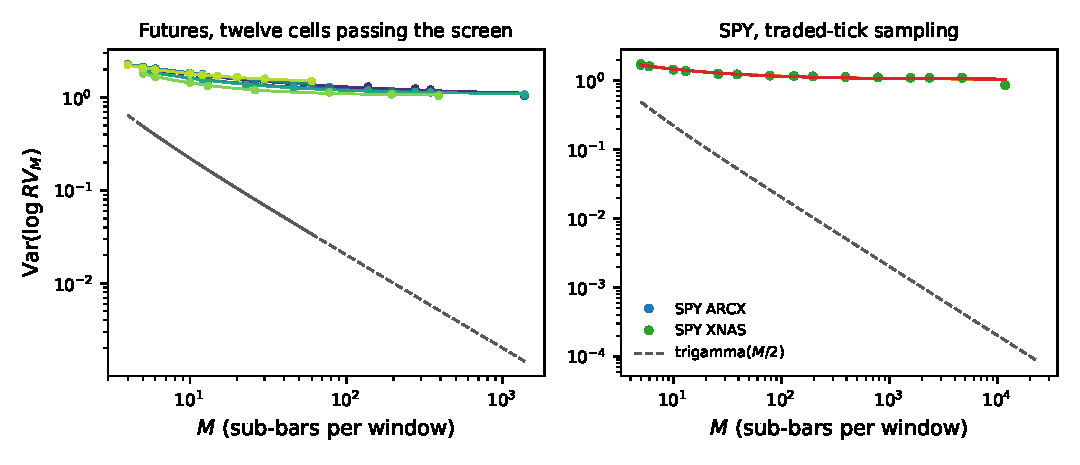
\includegraphics[width=\textwidth]{fig1.pdf}
\caption{$\operatorname{Var}(\log RV_M)$ against $M$ on log axes. Left: the twelve futures cells passing the tightened screen, points read from
\texttt{s08-final/results/phase4\_lambda.csv} and fitted curves from
\texttt{s10-exponent-audit/results/phase1\_bootstrap.csv}. Right: both SPY venues
under traded-tick sampling, points from
\texttt{s07-completion-and-spy/results/phase6\_spy\_grid\_\{ARCX,XNAS\}.csv}.
Dashed lines are trigamma$(M/2)$ on each grid. Twelve futures cells and two SPY
venues pass the screen, fourteen in total; the twelve futures cells are six
distinct cells under two boundary treatments that give identical fits.}
\label{fig:scaling}
\end{figure}
\begin{figure}[htbp]\centering
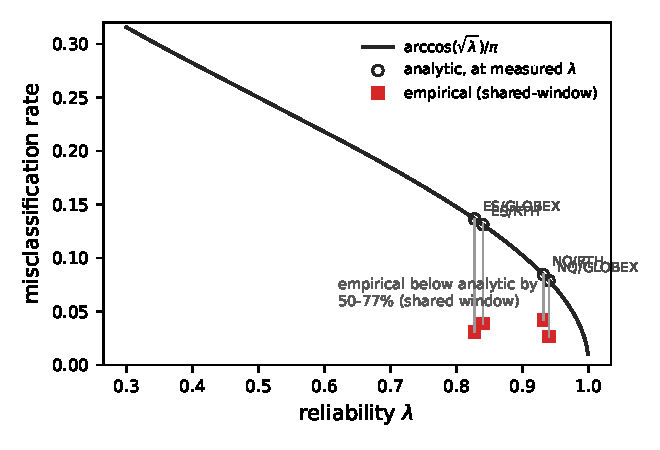
\includegraphics[width=0.62\textwidth]{fig2.pdf}
\caption{Misclassification against reliability. The curve is
$\arccos(\sqrt{\lambda})/\pi$. Open circles mark the analytic rate at each cell's
measured $\lambda$; squares mark the empirical rate against a finest-grid
noise-robust proxy, which is a lower bound because the two series share a window.
Read from \texttt{s14-applications/results/phase1\_k8\_rates.csv} and
\texttt{s09-application/results/phase3\_sizing\_params.csv}.}
\label{fig:mis}
\end{figure}
\clearpage
\bibliographystyle{plainnat}
\bibliography{refs}
\end{document}
